\chapter{État de l'art}

\rhead{État de l'art}
\lfoot{\leftmark}

\section{Introduction}
Ce chapitre dresse un panorama critique des technologies, des paradigmes et des travaux de recherche qui constituent le fondement théorique et pratique de notre projet. L'automatisation du triage de tickets logiciels est un problème à l'intersection de plusieurs domaines : l'ingénierie des données à grande échelle, le traitement automatique du langage naturel, l'apprentissage automatique et les architectures cloud modernes. Notre démarche suit une progression logique : nous commençons par définir les enjeux du Big Data et des architectures de stockage, avant de passer en revue les outils de transformation et d'orchestration, puis d'approfondir les fondements de l'intelligence artificielle appliquée au texte. Nous présentons ensuite le paradigme RAG (Retrieval-Augmented Generation) et les approches de classification de tickets dans la littérature, pour conclure par une synthèse comparative justifiant les choix technologiques retenus.

%--------------------------1-----------------------------
\section{Le Big Data : concepts et enjeux}

\subsection{Définition et caractéristiques}

Le Big Data \cite{logo:BG} désigne des ensembles de données dont le volume, la vélocité et la variété dépassent les capacités des outils traditionnels de gestion de l'information. Ces données proviennent de sources hétérogènes : réseaux sociaux, capteurs connectés, transactions financières, systèmes de gestion de tickets, journaux applicatifs, etc. L'enjeu fondamental n'est pas simplement de stocker ces volumes, mais d'en extraire de la valeur de manière fiable et reproductible.

La communauté scientifique et industrielle a progressivement enrichi la définition initiale à trois V (Volume, Vitesse, Variété) pour aboutir à un cadre à sept dimensions, illustré en figure \ref{fig:7v}, qui rend mieux compte de la complexité réelle des systèmes de données modernes \cite{logo:7v} :

\begin{itemize}
    \item \textbf{Volume :} La quantité de données générées croît de manière exponentielle. IDC estime que le volume mondial de données atteindra 175 zettaoctets d'ici 2025 \cite{logo:idc2021}, imposant des infrastructures de stockage distribuées.
    \item \textbf{Vitesse (Velocity) :} La fréquence de génération et de traitement des données varie du temps réel (flux de capteurs IoT) au traitement différé (analyses nocturnes). Les architectures modernes doivent gérer les deux régimes.
    \item \textbf{Variété (Variety) :} Les données sont structurées (tables relationnelles), semi-structurées (JSON, XML, YAML) ou non structurées (texte libre, images, vidéos, audio). La gestion de cette hétérogénéité constitue un défi majeur de l'ingénierie des données.
    \item \textbf{Véracité (Veracity) :} La qualité, la cohérence et la fiabilité des données ne peuvent être tenues pour acquises. Des données incomplètes, contradictoires ou biaisées conduisent à des analyses erronées et à des décisions inappropriées.
    \item \textbf{Valeur (Value) :} La finalité ultime est de transformer les données brutes en connaissance exploitable. Cette transformation nécessite des processus de nettoyage, d'agrégation, de modélisation et de visualisation rigoureux.
    \item \textbf{Variabilité (Variability) :} Les données peuvent changer de signification ou de format selon le contexte ou le moment de leur collecte, compliquant leur interprétation et leur traitement automatisé.
    \item \textbf{Visibilité (Visibility) :} La capacité à rendre les données compréhensibles et accessibles aux parties prenantes, qu'elles soient techniques ou métier, est une condition sine qua non de leur valorisation.
\end{itemize}

\begin{figure}[H]
    \centering
    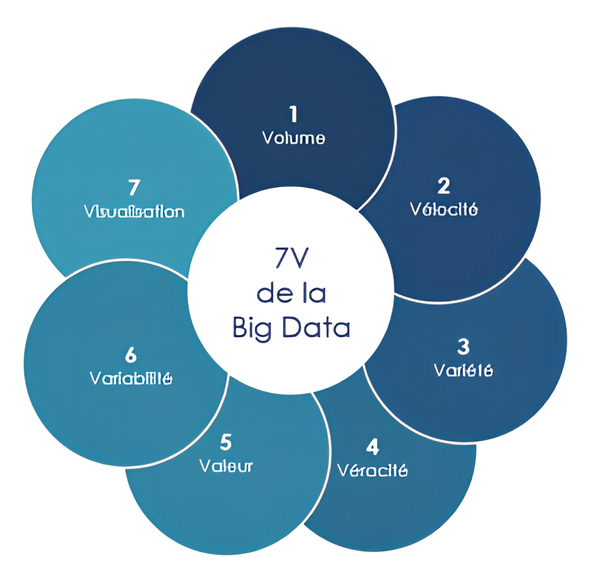
\includegraphics[width=0.55\textwidth]{images/7v.png}
    \caption{Les 7 V du Big Data}
    \label{fig:7v}
\end{figure}

\subsection{Enjeux spécifiques au projet}

Dans le contexte du triage automatique de tickets JIRA, le Big Data se manifeste à travers plusieurs enjeux concrets. Le premier est d'ordre volumétrique : le corpus Apache Spark totalise près de 50 000 tickets, chacun accompagné de commentaires, d'un journal de modifications et de relations inter-tickets, produisant plusieurs millions d'enregistrements à ingérer et transformer.

Le second enjeu est la variété des données. Les tickets combinent des données structurées (statut, priorité, dates, identifiants), des données semi-structurées (métadonnées JSON de l'API JIRA) et des données non structurées (descriptions textuelles, commentaires en langage naturel). Leur traitement conjoint exige une architecture unifiée capable de gérer ces formats hétérogènes.

Le troisième enjeu est celui de la qualité et de la véracité. Les descriptions de tickets varient considérablement en longueur, en langue (anglais, français, termes techniques mixtes) et en précision. Certains champs sont absents ou incohérents. Un processus de nettoyage et de normalisation rigoureux est indispensable pour alimenter un pipeline de classification fiable.

Enfin, la valeur produite doit être tangible et directement exploitable par les équipes opérationnelles : prédictions de catégorie, estimation de la résolution probable et résumés correctifs actionnables.

%------------------------2--------------------------
\section{Architectures de stockage et de traitement des données}

\subsection{Du Data Warehouse traditionnel au Cloud Data Warehouse}

Le concept d'entrepôt de données (Data Warehouse) remonte aux travaux fondateurs de William Inmon \cite{logo:inmon} et Ralph Kimball \cite{logo:kimball} dans les années 1990. Un entrepôt de données est un référentiel centralisé conçu pour le reporting et l'analyse, alimenté par des processus ETL (Extract, Transform, Load) qui transforment les données opérationnelles en structures optimisées pour la lecture. Les systèmes traditionnels tels qu'Oracle Exadata ou Teradata ont longtemps dominé ce marché, mais ils souffrent de limitations importantes face aux volumes du Big Data : coût élevé des licences, scalabilité limitée et rigidité architecturale.

L'avènement du cloud computing a profondément modifié ce paysage en permettant l'émergence de solutions élastiques, facturées à l'usage et capables de traiter des pétaoctets de données. Ces plateformes cloud modernes dissocient généralement le stockage du calcul, permettant de dimensionner chaque ressource indépendamment selon les besoins.

\subsection{Panorama des plateformes cloud modernes}

\paragraph{Snowflake}

Snowflake \cite{logo:snowflake} est une plateforme de données cloud conçue dès l'origine pour le cloud, sans héritage d'architecture on-premise. Son architecture tri-couche, illustrée en figure \ref{fig:snowflake_archi}, sépare les services cloud (méta-données, sécurité, authentification), le calcul (entrepôts virtuels indépendants) et le stockage (S3, Azure Blob, GCS selon le cloud hôte). Cette séparation confère à Snowflake une élasticité remarquable : il est possible d'exécuter plusieurs charges de travail simultanément sur les mêmes données sans contention de ressources.

Snowflake prend nativement en charge le SQL ANSI, les données semi-structurées au format JSON (via le type \texttt{VARIANT}), le clonage instantané de tables sans duplication de données, et le partage sécurisé de données entre organisations. Sa couche d'intelligence artificielle intégrée, Snowflake Cortex, est détaillée dans la section~\ref{sec:cortex}.

\begin{figure}[H]
\centering
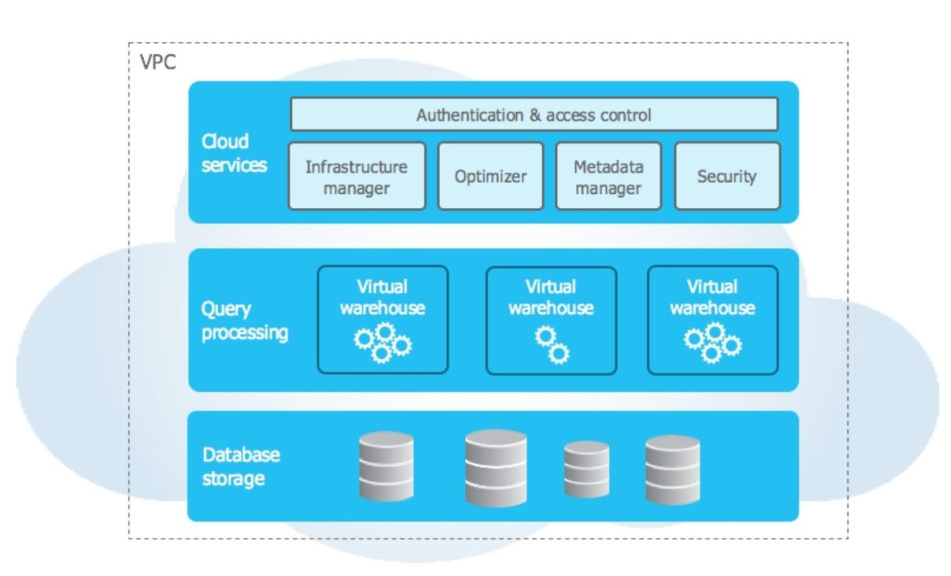
\includegraphics[width=0.85\textwidth]{images/archisnwoflake.png}
\caption{Architecture de Snowflake : séparation stockage, calcul et services}
\label{fig:snowflake_archi}
\end{figure}

\paragraph{Google BigQuery}

Google BigQuery \cite{logo:bigquery} est l'entrepôt de données serverless de Google Cloud Platform. Il repose sur le moteur de traitement Dremel, qui découpe automatiquement les requêtes en tâches parallèles exécutées sur des milliers de nœuds. BigQuery stocke les données en format colonne compressé sur le système de fichiers Colossus de Google, garantissant des performances élevées sur les requêtes analytiques portant sur de grandes plages temporelles. Il intègre BigQuery ML pour l'entraînement et l'inférence de modèles directement depuis SQL, ainsi que des connecteurs natifs vers les services d'IA de Google (Vertex AI \cite{logo:vertex_ai}).

\paragraph{Amazon Redshift}

Amazon Redshift \cite{logo:redshift} est le service d'entrepôt de données managé d'AWS. Il repose sur une architecture MPP (Massively Parallel Processing) et stocke les données en colonnes compressées sur des nœuds de calcul. Redshift Spectrum permet d'interroger des données stockées sur S3 sans les charger dans l'entrepôt. Redshift ML offre une intégration avec Amazon SageMaker pour l'entraînement automatique de modèles. Sa profonde intégration dans l'écosystème AWS en fait un choix naturel pour les organisations déjà investies dans cette infrastructure.

\paragraph{Azure Synapse Analytics}

Azure Synapse Analytics \cite{logo:synapse} est la solution unifiée de Microsoft combinant entrepôt de données analytiques et traitement Big Data. Il permet d'interroger indifféremment des données stockées dans Azure Data Lake Storage via SQL serverless ou dans des pools SQL dédiés. Son intégration avec Azure Machine Learning, Azure OpenAI Service et Power BI en fait une plateforme bout-en-bout pour les organisations de l'écosystème Microsoft.

\subsection{L'architecture Lakehouse}

L'architecture Lakehouse \cite{logo:databricks}, popularisée par Databricks, cherche à réunir les avantages complémentaires du data lake (stockage flexible et peu coûteux de données brutes dans des formats ouverts) et du data warehouse (performances analytiques, garanties transactionnelles, gouvernance). La figure \ref{fig:lakehouse_archi} illustre cette architecture hybride.

\begin{figure}[H]
\centering
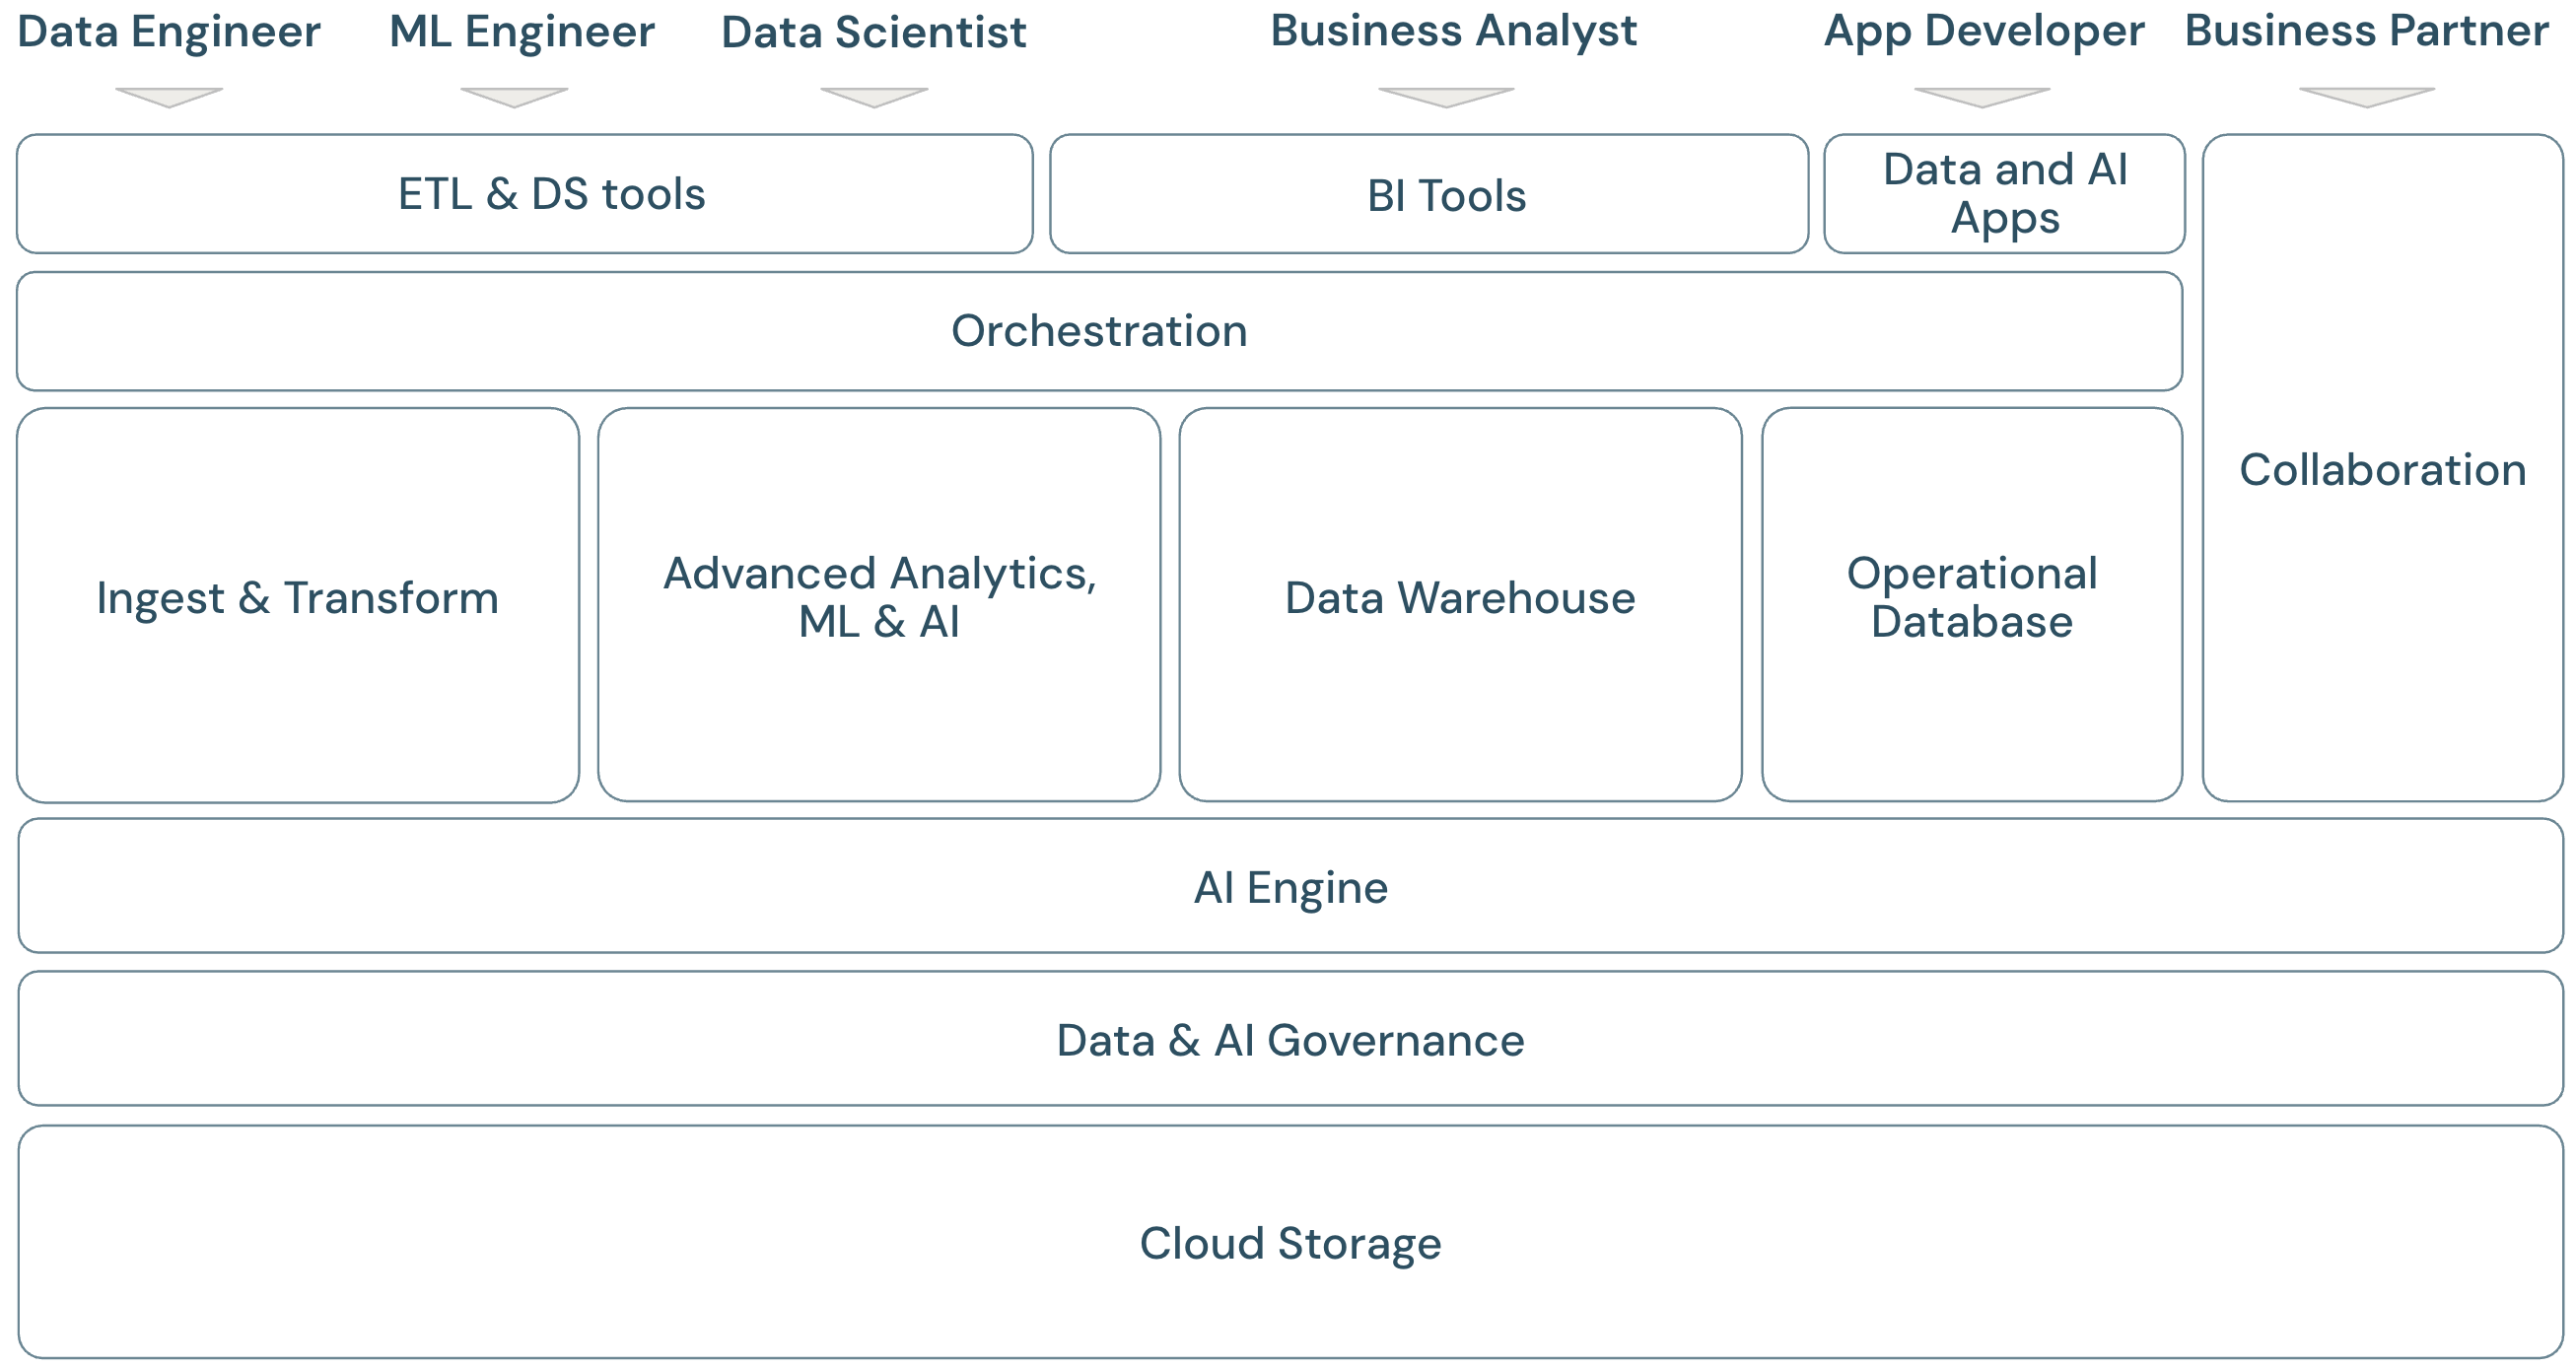
\includegraphics[width=0.85\textwidth]{images/lakehouse_architecture.png}
\caption{Architecture Lakehouse selon Databricks}
\label{fig:lakehouse_archi}
\end{figure}

Le format ouvert Delta Lake constitue la pierre angulaire de cette architecture : il ajoute une couche transactionnelle conforme aux propriétés ACID au-dessus de fichiers Parquet stockés dans un data lake. D'autres formats ouverts comme Apache Iceberg ou Apache Hudi répondent à des objectifs similaires et connaissent une adoption croissante. Databricks construit au-dessus de cette fondation une plateforme unifiée pour l'ingénierie des données (pipelines Spark), la data science et l'analyse SQL.

\subsection{Tableau comparatif des plateformes}

Le tableau \ref{tab:comparatif_dw} synthétise les caractéristiques des principales plateformes selon les critères pertinents pour notre projet.

\begin{table}[h!]
\centering
\begin{tabularx}{\textwidth}{|l|X|X|X|X|}
  \hline
  \textbf{Critère} & \textbf{Snowflake} & \textbf{BigQuery} & \textbf{Redshift} & \textbf{Databricks} \\
  \hline
  Modèle de facturation & Crédits (stockage + calcul séparés) & À la requête ou forfait & Instance réservée & DBU (unité de traitement) \\
  \hline
  Multi-cloud natif & Oui (AWS, GCP, Azure) & Non (GCP) & Non (AWS) & Oui \\
  \hline
  Formats semi-structurés & Natif (VARIANT) & Natif & Via Spectrum & Via Delta Lake \\
  \hline
  IA intégrée & Cortex (LLM, embeddings) & BigQuery ML, Vertex AI & SageMaker & MLflow, Model Serving \\
  \hline
  Architecture & Séparation calcul/stockage & Serverless & MPP & Lakehouse (Spark) \\
  \hline
  Conformité données & Élevée (données dans Snowflake) & GCP (certifications SOC2) & AWS (certifications SOC2) & Dépend du cloud hôte \\
  \hline
\end{tabularx}
\caption{Comparaison des principales plateformes de données cloud}
\label{tab:comparatif_dw}
\end{table}

%------------------------3--------------------------
\section{Outils de transformation et d'orchestration des données}

\subsection{Le paradigme ELT et les outils de transformation}

L'ingénierie des données repose traditionnellement sur le paradigme ETL (Extract, Transform, Load), où les transformations sont effectuées dans un moteur intermédiaire avant chargement dans l'entrepôt. L'avènement des entrepôts cloud puissants a favorisé l'émergence du paradigme ELT (Extract, Load, Transform), dans lequel les données brutes sont chargées dans l'entrepôt avant d'y être transformées en exploitant directement sa puissance de calcul. Cette inversion simplifie l'architecture et améliore les performances pour les transformations analytiques.

\paragraph{dbt (Data Build Tool)}

dbt \cite{logo:dbt} est l'outil de référence du paradigme ELT moderne. Il applique les principes du génie logiciel au travail de transformation de données : les modèles sont versionnés, testés, documentés et organisés en graphe acyclique dirigé (DAG) garantissant un ordre d'exécution correct et une reproductibilité totale. La figure \ref{fig:dbt_workflow} illustre le fonctionnement de dbt.

\begin{figure}[H]
\centering
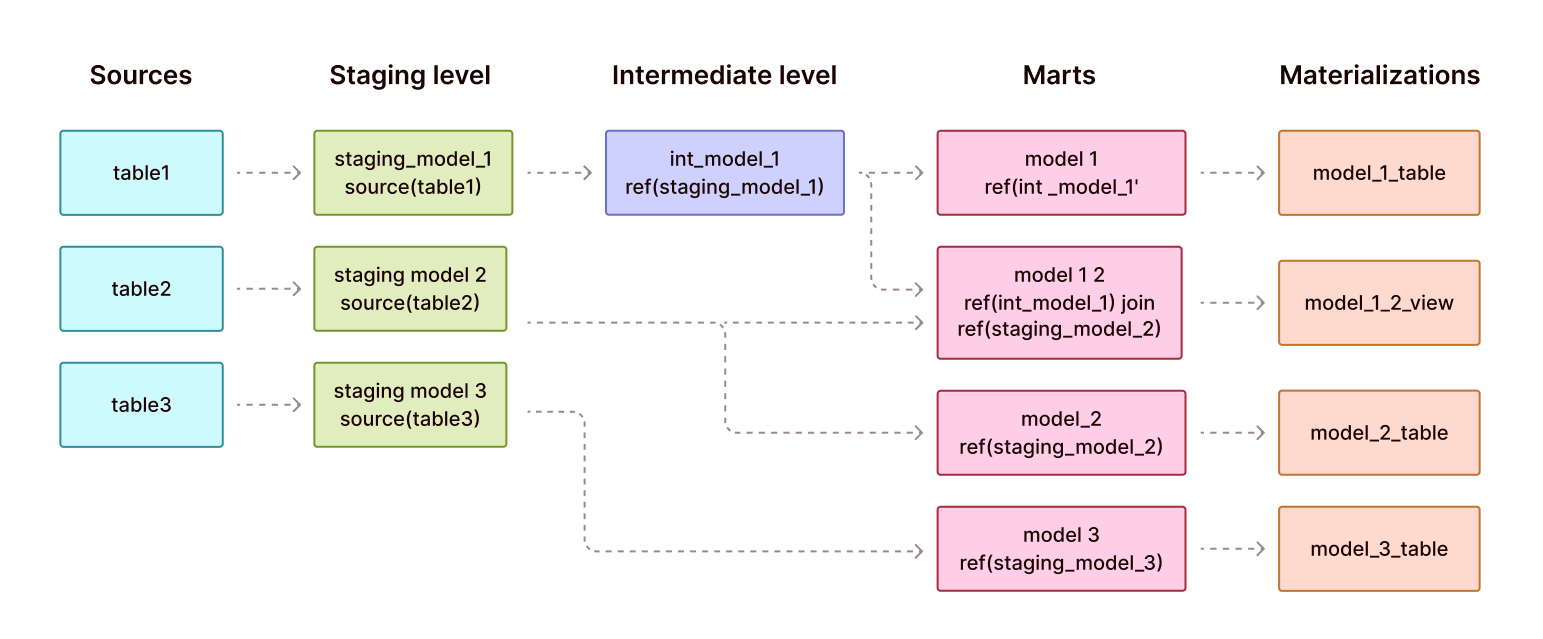
\includegraphics[width=0.85\textwidth]{images/dbt_workflow.png}
\caption{Fonctionnement de dbt : transformations SQL orchestrées dans l'entrepôt}
\label{fig:dbt_workflow}
\end{figure}

Chaque modèle dbt est un fichier SQL représentant une transformation. dbt génère le code d'exécution approprié (création de vues ou de tables matérialisées) et le soumet directement à l'entrepôt. Les tests intégrés permettent de valider automatiquement l'unicité des clés, l'absence de valeurs nulles inattendues, les plages de valeurs admissibles et les relations référentielles. La documentation est générée automatiquement à partir des modèles et des métadonnées associées.

\paragraph{Talend}

Talend \cite{logo:talend} est une plateforme d'intégration de données qui propose une approche ETL graphique. Ses composants préconfigurés permettent de concevoir des pipelines sans écrire de code, ce qui la rend accessible aux profils non développeurs. Talend dispose de nombreux connecteurs vers les sources de données hétérogènes. Cependant, sa complexité opérationnelle, son modèle de licence et ses performances sur de très grands volumes en font un outil moins adapté aux architectures ELT modernes.

\paragraph{Apache NiFi}

Apache NiFi \cite{logo:nifi} est une plateforme d'automatisation des flux de données, particulièrement adaptée à l'ingestion en temps réel depuis des sources hétérogènes. Son interface visuelle permet de construire des pipelines drag-and-drop, et son architecture distribuée assure une haute disponibilité. NiFi excelle pour l'ingestion et le routage de flux, mais ses capacités de transformation analytique restent limitées comparées aux outils ELT dédiés.

\subsection{L'orchestration des workflows de données}

L'orchestration désigne la planification, la surveillance et la gestion des dépendances entre les tâches composant un pipeline de données. Elle répond à la nécessité de gérer des workflows complexes avec des dépendances, des reprises sur erreur, des notifications et une observabilité complète.

\paragraph{Apache Airflow}

Apache Airflow \cite{logo:airflow} est l'orchestrateur de workflows open source le plus répandu dans l'écosystème de données. Les pipelines sont définis en Python sous forme de DAG, offrant une expressivité totale. Airflow dispose d'une interface web riche pour la surveillance et d'un écosystème important de connecteurs (opérateurs) vers les systèmes externes. La figure \ref{fig:airflow_dag} illustre un exemple de DAG dans Airflow.

\begin{figure}[H]
\centering
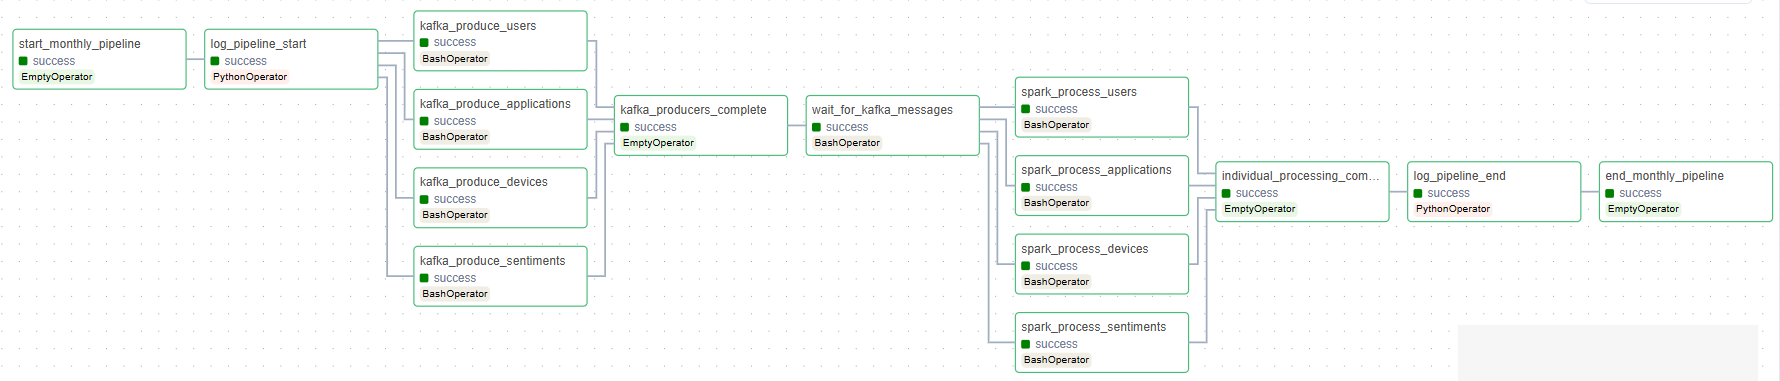
\includegraphics[width=0.85\textwidth]{images/airflow_dag.png}
\caption{Exemple de DAG dans Apache Airflow}
\label{fig:airflow_dag}
\end{figure}

\paragraph{Prefect et Dagster}

Prefect \cite{logo:prefect} et Dagster \cite{logo:dagster} sont des orchestrateurs de nouvelle génération qui répondent à certaines limitations d'Airflow. Prefect met l'accent sur la résilience et la testabilité des workflows, avec une approche orientée flux de données. Dagster introduit le concept d'asset software-defined, où l'orchestration est centrée non plus sur les tâches mais sur les données produites, facilitant la traçabilité et la gestion des dépendances dans les grands projets de données.

\subsection{Tableau comparatif des outils de transformation et d'orchestration}

\begin{table}[h!]
\centering
\begin{tabularx}{\textwidth}{|l|X|X|X|}
  \hline
  \textbf{Critère} & \textbf{dbt} & \textbf{Talend} & \textbf{Apache NiFi} \\
  \hline
  Paradigme & ELT (SQL dans l'entrepôt) & ETL (moteur externe) & Ingestion/flux \\
  \hline
  Courbe d'apprentissage & Faible (SQL) & Moyenne (interface graphique) & Moyenne \\
  \hline
  Tests et qualité & Intégrés nativement & Partiels & Limités \\
  \hline
  Documentation auto & Oui (DAG interactif) & Partielle & Non \\
  \hline
  Adapté à ELT cloud & Oui & Non & Non \\
  \hline
  Open source & Oui (Core) & Partiellement & Oui \\
  \hline
\end{tabularx}
\caption{Comparaison des outils de transformation de données}
\label{tab:comparatif_transformation}
\end{table}

%------------------------4--------------------------
\section{Intelligence artificielle appliquée au traitement du texte}

\subsection{Évolution du traitement automatique du langage naturel}

Le traitement automatique du langage naturel (TALN, ou NLP en anglais) est la discipline de l'intelligence artificielle qui s'intéresse à la compréhension et à la génération du langage humain par les machines. Appliqué à la classification de tickets logiciels, le NLP permet d'analyser automatiquement le contenu textuel des descriptions d'incidents pour en inférer la catégorie, la priorité et la résolution probable.

\subsubsection{Approches classiques : représentations vectorielles creuses}

Les premières approches de classification de texte reposaient sur des représentations vectorielles creuses. Le modèle sac-de-mots (bag-of-words) représente chaque document comme un vecteur dont les composantes correspondent aux fréquences des termes du vocabulaire, indépendamment de leur ordre d'apparition. La pondération TF-IDF (Term Frequency–Inverse Document Frequency) \cite{logo:tfidf} raffine cette représentation en diminuant le poids des termes fréquents dans l'ensemble du corpus (déterminants, verbes courants) et en valorisant les termes discriminants.

Ces représentations alimentent des classifieurs statistiques éprouvés : machines à vecteurs de support (SVM), forêts aléatoires (Random Forests), régression logistique, classifieurs naïfs de Bayes. Ces méthodes ont produit des résultats satisfaisants sur les corpus de petite taille et les tâches simples. Cependant, elles souffrent de deux limitations fondamentales : elles ne capturent pas la sémantique des termes (deux mots synonymes sont traités comme distincts), et la haute dimensionnalité des vecteurs creuses pose des problèmes de généralisation et de complexité computationnelle.

\subsubsection{Représentations distribuées : l'ère des word embeddings}

L'introduction des représentations distribuées a constitué une rupture paradigmatique dans le TALN. L'idée fondatrice, issue de l'hypothèse distributionnelle de Harris (1954), est que le sens d'un mot peut être inféré de son contexte d'apparition. Des mots apparaissant dans des contextes similaires ont des représentations vectorielles proches dans l'espace d'embedding.

\paragraph{Word2Vec}

Word2Vec \cite{logo:word2vec}, proposé par Mikolov et al. (2013) chez Google, est le premier modèle d'embedding à grande échelle à démontrer l'utilité pratique des représentations distribuées. Il repose sur deux architectures d'entraînement complémentaires : le modèle CBOW (Continuous Bag-of-Words), qui prédit un mot à partir des mots de son contexte, et le modèle Skip-gram, qui prédit les mots du contexte à partir du mot central. Word2Vec produit des représentations vectorielles denses de quelques centaines de dimensions qui capturent des analogies sémantiques remarquables.

La principale limite de Word2Vec est son caractère statique : chaque mot reçoit un vecteur unique, quelle que soit sa polysémie. Le terme \textit{« banque »} possède le même vecteur qu'il désigne un établissement financier ou la rive d'un cours d'eau.

\paragraph{GloVe}

GloVe (Global Vectors for Word Representation) \cite{logo:glove}, proposé par Pennington et al. (2014) à Stanford, adopte une approche différente : il factorise la matrice de co-occurrence globale du corpus pour produire des embeddings capturant à la fois les statistiques locales et globales du langage. GloVe offre des performances comparables à Word2Vec sur de nombreuses tâches, avec un entraînement plus efficace sur de grands corpus.

\paragraph{ELMo}

ELMo (Embeddings from Language Models) \cite{logo:elmo}, proposé par Peters et al. (2018), introduit des représentations contextuelles au niveau du mot. Le vecteur d'un terme est calculé dynamiquement en fonction de son contexte phrastique, résolvant ainsi le problème de polysémie. ELMo repose sur des réseaux récurrents LSTM bidirectionnels pré-entraînés sur de larges corpus textuels.

\subsubsection{La révolution Transformer}

L'architecture Transformer \cite{logo:transformer}, proposée par Vaswani et al. en 2017 dans l'article fondateur \textit{Attention is All You Need}, a profondément transformé le domaine du TALN et au-delà. Son mécanisme central, l'auto-attention (self-attention), permet au modèle de pondérer dynamiquement l'importance de chaque élément d'une séquence par rapport à tous les autres éléments, capturant ainsi les dépendances à longue portée sans les limitations des architectures récurrentes.

À la différence des réseaux de neurones récurrents (RNN, LSTM), qui traitent les séquences de manière séquentielle et peinent à propager l'information sur de longues distances, le Transformer traite tous les éléments de la séquence en parallèle. Cela permet un entraînement plus efficace sur des corpus massifs et une meilleure capture des dépendances sémantiques complexes.

Le mécanisme d'attention multi-têtes permet au modèle de capturer simultanément différents types de relations entre les tokens (relations syntaxiques, coréférentielles, sémantiques), en calculant l'attention selon plusieurs sous-espaces de représentation indépendants dont les résultats sont ensuite concaténés.

\subsection{Les modèles pré-entraînés et le paradigme du transfert d'apprentissage}

\subsubsection{BERT et ses dérivés}

BERT (Bidirectional Encoder Representations from Transformers) \cite{logo:bert}, proposé par Devlin et al. (2018) chez Google, a inauguré l'ère des modèles de langage pré-entraînés à grande échelle. BERT est un encodeur Transformer bidirectionnel pré-entraîné sur deux tâches non supervisées : la prédiction de mots masqués (Masked Language Modeling) et la prédiction de la relation entre deux phrases consécutives (Next Sentence Prediction). Ce pré-entraînement sur de vastes corpus (BooksCorpus et Wikipedia anglaise) lui confère une représentation riche et généraliste du langage.

L'apport majeur de BERT est le paradigme pré-entraînement/fine-tuning : un modèle BERT pré-entraîné peut être adapté à une tâche spécifique (classification, extraction d'entités, question-réponse) en ajoutant une couche de prédiction et en réentraînant l'ensemble sur un petit corpus annoté. Cette approche a établi de nouveaux records de performance sur la quasi-totalité des benchmarks NLP de l'époque.

De nombreux modèles dérivés ont suivi : RoBERTa \cite{logo:roberta} (Meta, entraînement optimisé avec davantage de données), DistilBERT (modèle allégé par distillation de connaissance), CamemBERT pour le français, DeBERTa (Microsoft, mécanisme d'attention décorrelé). Chacun apporte des améliorations sur des aspects spécifiques tout en conservant l'architecture encodeur bidirectionnelle de BERT.

\subsubsection{Les modèles d'embedding de phrases}

La classification de tickets requiert non pas des embeddings au niveau du mot, mais des représentations vectorielles de phrases ou de paragraphes entiers. La bibliothèque \texttt{sentence-transformers} \cite{logo:sentence_transformers}, proposée par Reimers et Gurevych (2019), adapte les modèles BERT à cette tâche via un entraînement par paires de phrases similaires et dissimilaires (apprentissage contrastif siamois). Ce paradigme d'entraînement assure que des phrases sémantiquement proches produisent des embeddings proches dans l'espace vectoriel.

Parmi les modèles d'embedding de référence, on distingue :
\begin{itemize}
    \item \textbf{all-MiniLM-L6-v2 \cite{logo:sentence_transformers} :} Un modèle compact offrant un bon équilibre entre qualité des embeddings (384 dimensions) et vitesse d'inférence sur CPU. Particulièrement adapté aux environnements contraints en ressources computationnelles.
    \item \textbf{E5 (Microsoft) \cite{logo:e5} :} Une famille de modèles optimisés pour la recherche sémantique et le reranking, entraînés sur de vastes corpus de paires textuelles.
    \item \textbf{voyage-multilingual-2 (Voyage AI) \cite{logo:snowflake_cortex} :} Un modèle multilingue de haute performance couvrant plus de 30 langues, particulièrement adapté aux corpus techniques comportant des termes issus de plusieurs langues.
    \item \textbf{text-embedding-3-large (OpenAI) \cite{logo:openai} :} Un modèle propriétaire accessible via API, produisant des vecteurs de 3072 dimensions avec des performances de pointe sur les benchmarks MTEB.
\end{itemize}

\subsection{Les grands modèles de langage}

\subsubsection{Définition et principes fondamentaux}

Les grands modèles de langage (LLM, Large Language Models) sont des modèles Transformer pré-entraînés sur des corpus textuels massifs comptant des centaines de milliards de tokens, avec des paramètres se chiffrant en milliards. Leur pré-entraînement via des objectifs auto-supervisés (modélisation du langage causal ou masqué) leur confère une connaissance généraliste du langage et du monde, exploitable sans réentraînement par simple formulation de la tâche dans un prompt : c'est le principe du zero-shot et du few-shot learning.

Les LLM modernes surpassent les approches précédentes sur une vaste gamme de tâches : compréhension de texte, génération de contenu structuré, raisonnement, extraction d'informations, traduction, résumé et classification. Leur capacité à traiter des fenêtres de contexte de plus en plus larges (jusqu'à plusieurs centaines de milliers de tokens pour les modèles récents) leur permet d'intégrer des instructions détaillées et des exemples directement dans le prompt.

\subsubsection{Panorama des principales familles de LLM}

\paragraph{La famille GPT (OpenAI)}

La série GPT (Generative Pre-trained Transformer) \cite{logo:openai} représente l'évolution la plus emblématique des modèles auto-régressifs génératifs. GPT-3 (2020) a démontré pour la première fois les capacités de few-shot learning à grande échelle. GPT-4 et ses déclinaisons (GPT-4o, GPT-4 Turbo) ont ensuite établi de nouveaux standards en matière de raisonnement, de compréhension contextuelle et de génération de code. Ces modèles sont accessibles via l'API OpenAI et sont particulièrement performants pour les tâches de génération de contenu structuré et de raisonnement complexe.

\paragraph{La famille Claude (Anthropic)}

La famille Claude \cite{logo:anthropic_api} est développée par Anthropic selon des principes d'alignement rigoureux. Claude se distingue par sa fenêtre de contexte étendue (jusqu'à 200 000 tokens pour Claude 3 Opus), sa précision sur les tâches d'analyse de texte long, et son orientation vers la sécurité et la fiabilité des sorties. La conception de ces modèles intègre des techniques d'apprentissage par renforcement à partir du retour humain (RLHF) et d'apprentissage constitutionnel (Constitutional AI), réduisant les sorties nuisibles ou inappropriées.

\paragraph{La famille Llama (Meta)}

Meta AI propose avec la famille Llama \cite{logo:llama} des modèles à poids ouverts (open weights), permettant un déploiement local ou dans des environnements cloud maîtrisés sans transmission de données vers des tiers. Llama 3, avec ses variantes de 8B et 70B paramètres, offre des performances comparables aux modèles propriétaires sur de nombreuses tâches de compréhension et de génération, tout en préservant la confidentialité des données sensibles.

\paragraph{La famille Mistral}

Mistral AI, société française fondée en 2023, a rapidement acquis une réputation d'excellence dans le domaine des LLM efficaces. Le modèle Mistral 7B \cite{logo:mistral} a démontré que des modèles de taille modérée, entraînés avec soin, peuvent rivaliser avec des modèles bien plus grands. Mistral Large 2 est particulièrement reconnu pour son rapport performances/coût favorable et ses capacités en contexte multilingue. Son architecture intègre des mécanismes d'attention à fenêtre glissante (sliding window attention) et de regroupement de têtes d'attention (grouped-query attention) qui optimisent l'efficacité computationnelle.

\subsubsection{Stratégies d'utilisation des LLM}

Plusieurs stratégies permettent d'exploiter les LLM selon les contraintes et les objectifs du projet :

\begin{itemize}
    \item \textbf{Zero-shot prompting :} Le modèle est sollicité directement sur la tâche sans exemple préalable. Cette approche exploite la connaissance générale acquise lors du pré-entraînement. Elle est simple à mettre en œuvre mais peut manquer de précision sur des tâches très spécifiques à un domaine.

    \item \textbf{Few-shot prompting :} Quelques exemples représentatifs de la tâche sont fournis dans le prompt pour guider le modèle. Les exemples agissent comme des démonstrations in-context qui orientent le format et le contenu de la réponse. Cette approche améliore significativement la précision sans nécessiter de réentraînement.

    \item \textbf{Chain-of-thought prompting :} Le modèle est invité à détailler son raisonnement étape par étape avant de formuler sa réponse. Cette technique, proposée par Wei et al. \cite{logo:cot}, améliore les performances sur les tâches requérant un raisonnement multi-étapes, au prix d'une latence et d'un coût en tokens plus élevés.

    \item \textbf{Fine-tuning supervisé :} Le modèle pré-entraîné est réentraîné sur un corpus annoté spécifique à la tâche. Cette approche offre les meilleures performances sur le domaine cible, mais nécessite des données annotées de qualité, une infrastructure GPU dédiée et une expertise en entraînement de modèles.

    \item \textbf{Retrieval-Augmented Generation (RAG) :} Le modèle est enrichi dynamiquement avec des informations pertinentes récupérées depuis une base de connaissances externe au moment de l'inférence. Cette approche est détaillée dans la section suivante.
\end{itemize}

%------------------------5--------------------------
\section{La recherche sémantique et les bases de données vectorielles}

\subsection{Principe de la recherche vectorielle}

La recherche vectorielle repose sur la représentation des documents sous forme de vecteurs denses dans un espace de haute dimension, puis sur l'identification des vecteurs les plus proches d'une requête selon une mesure de similarité donnée. Contrairement à la recherche par mots-clés (qui requiert une correspondance exacte de termes), la recherche vectorielle capture la proximité sémantique : deux textes exprimant la même idée avec des termes différents se retrouvent proches dans l'espace d'embedding.

\subsection{Mesures de similarité vectorielle}

Le choix de la mesure de similarité influe sur la qualité des résultats de recherche. Les trois mesures les plus utilisées sont :

\begin{itemize}
    \item \textbf{Similarité cosinus :} Mesure l'angle entre deux vecteurs, indépendamment de leur norme. C'est la mesure de référence pour les embeddings de texte, car elle est invariante à la longueur du document. Elle retourne une valeur entre $-1$ et $1$, où $1$ indique une orientation identique dans l'espace vectoriel.

    \item \textbf{Distance euclidienne (L2) :} Mesure la distance géométrique entre deux points dans l'espace vectoriel. Contrairement à la similarité cosinus, elle est sensible à la norme des vecteurs et peut être affectée par les variations de longueur des textes.

    \item \textbf{Produit scalaire (inner product) :} Prend en compte à la fois l'angle et la magnitude des vecteurs. Utilisé lorsque la norme du vecteur encode une information de pertinence, notamment dans certains systèmes de recommandation.
\end{itemize}

La recherche des $k$ plus proches voisins ($k$-NN) consiste à retrouver, parmi un corpus de référence préalablement indexé, les $k$ vecteurs les plus similaires à un vecteur requête. Pour les corpus de grande taille, des algorithmes d'indexation approximative (Approximate Nearest Neighbor, ANN), tels que HNSW (Hierarchical Navigable Small World) \cite{logo:hnsw} ou FAISS (Facebook AI Similarity Search) \cite{logo:faiss}, permettent d'effectuer cette recherche en temps sous-linéaire avec un compromis acceptable sur la précision.

\subsection{Bases de données vectorielles}

L'essor des LLM et des applications de recherche sémantique a favorisé l'émergence d'une nouvelle catégorie de systèmes de gestion de données : les bases de données vectorielles \cite{logo:vector_db_survey}. Ces systèmes sont optimisés pour le stockage, l'indexation et la recherche efficace de vecteurs denses à haute dimension. Le tableau \ref{tab:vector_db} présente les principales solutions disponibles.

\begin{table}[h!]
\centering
\begin{tabularx}{\textwidth}{|l|X|X|X|}
  \hline
  \textbf{Solution} & \textbf{Type} & \textbf{Points forts} & \textbf{Limitations} \\
  \hline
  Pinecone \cite{logo:pinecone} & Service managé (cloud) & Facilité d'utilisation, scalabilité, faible latence & Coût élevé, dépendance fournisseur \\
  \hline
  Weaviate \cite{logo:weaviate} & Open source / cloud & Multimodal, GraphQL, modules IA & Complexité de déploiement \\
  \hline
  Chroma \cite{logo:chroma} & Open source (local) & Légèreté, intégration LangChain & Scalabilité limitée \\
  \hline
  pgvector \cite{logo:pgvector} & Extension PostgreSQL & Intégration SQL native, pas d'infra supplémentaire & Performances ANN limitées \\
  \hline
  Snowflake Cortex \cite{logo:snowflake_cortex} & Intégré à Snowflake & Aucune extraction de données, SQL natif & Ecosystème Snowflake uniquement \\
  \hline
  Qdrant \cite{logo:qdrant} & Open source / cloud & Haute performance, filtrage riche & Moins mature que Pinecone \\
  \hline
\end{tabularx}
\caption{Comparaison des bases de données vectorielles}
\label{tab:vector_db}
\end{table}

%------------------------6--------------------------
\section{Le paradigme RAG (Retrieval-Augmented Generation)}

\subsection{Motivation et principes}

Le paradigme RAG \cite{logo:rag}, introduit par Lewis et al. (2020) chez Facebook AI Research, répond à une limitation fondamentale des LLM : leur connaissance est figée au moment de l'entraînement et ne reflète pas les données spécifiques à un domaine ou à une organisation. Un LLM interrogé sur des incidents internes ou sur des connaissances très spécialisées risque de produire des réponses inventées (phénomène dit d'hallucination) car il n'a jamais été exposé à ces informations.

L'idée centrale du RAG est d'enrichir dynamiquement le prompt du modèle avec des documents pertinents récupérés depuis une base de connaissances externe au moment de l'inférence. Le modèle dispose ainsi d'un contexte factuel sur lequel appuyer sa réponse, réduisant drastiquement le risque d'hallucination et permettant une adaptation au domaine sans réentraînement.

\subsection{Architecture générale du RAG}

Un pipeline RAG s'articule autour de trois composantes principales :

\begin{enumerate}
    \item \textbf{Phase d'indexation (offline) :} Les documents de la base de référence sont encodés sous forme d'embeddings vectoriels et stockés dans une base de données vectorielle. Cette phase est exécutée une fois lors de l'initialisation du système, puis incrémentalement à chaque ajout de nouveaux documents.

    \item \textbf{Phase de récupération (online) :} Lorsqu'une requête arrive, elle est encodée par le même modèle d'embedding que celui utilisé lors de l'indexation. Les $k$ documents dont les vecteurs sont les plus proches du vecteur requête sont récupérés depuis la base vectorielle.

    \item \textbf{Phase de génération (online) :} Le LLM reçoit un prompt enrichi comprenant la requête originale et les documents récupérés, qu'il utilise comme contexte pour formuler sa réponse. La réponse est ainsi ancrée sur des faits concrets plutôt que sur les seules connaissances internes du modèle.
\end{enumerate}

\subsection{Variantes et évolutions du RAG}

La recherche a produit plusieurs variantes du RAG original qui améliorent ses performances selon des axes différents \cite{logo:advanced_rag} :

\begin{itemize}
    \item \textbf{RAG naïf :} L'implémentation basique décrite ci-dessus. Efficace pour des cas simples mais sensible à la qualité des documents récupérés.

    \item \textbf{RAG avancé (Advanced RAG) :} Intègre des étapes de pré-récupération (reformulation de la requête, décomposition en sous-questions) et de post-récupération (reranking des documents, filtrage par pertinence) pour améliorer la qualité du contexte fourni au LLM.

    \item \textbf{RAG modulaire :} Architecture plus flexible permettant d'échanger indépendamment les composantes d'indexation, de récupération et de génération, facilitant l'expérimentation et l'optimisation de chaque partie.

    \item \textbf{RAG hybride :} Combine la recherche vectorielle sémantique avec une recherche par mots-clés (BM25 ou similaire) pour bénéficier des avantages complémentaires des deux approches. La recherche sémantique capture la proximité de sens, tandis que la recherche lexicale capture les correspondances de termes techniques exacts.

    \item \textbf{GraphRAG (Microsoft) \cite{logo:graphrag} :} Enrichit la récupération avec des relations extraites sous forme de graphe de connaissance, permettant des raisonnements multi-sauts sur des informations reliées.
\end{itemize}

\subsection{RAG versus fine-tuning : analyse comparative}

Le choix entre RAG et fine-tuning est une décision architecturale fondamentale dans les projets d'IA appliquée. Le tableau \ref{tab:rag_vs_finetune} met en regard les deux approches selon les critères pertinents pour notre contexte.

\begin{table}[h!]
\centering
\begin{tabularx}{\textwidth}{|l|X|X|}
  \hline
  \textbf{Critère} & \textbf{RAG} & \textbf{Fine-tuning} \\
  \hline
  Données annotées requises & Non (documents non étiquetés suffisent) & Oui (paires entrée/sortie annotées) \\
  \hline
  Mise à jour des connaissances & Immédiate (ajout de documents) & Nécessite un réentraînement \\
  \hline
  Traçabilité des réponses & Élevée (sources identifiables) & Faible (connaissance internalisée) \\
  \hline
  Infrastructure requise & Base vectorielle + API LLM & GPU dédiés pour l'entraînement \\
  \hline
  Hallucinations & Réduites (ancrage factuel) & Persistantes si données insuffisantes \\
  \hline
  Coût de déploiement & Faible à moyen & Élevé (coût GPU) \\
  \hline
  Adaptation au domaine & Bonne & Excellente \\
  \hline
  Confidentialité des données & Élevée si base locale & Données exposées lors de l'entraînement \\
  \hline
\end{tabularx}
\caption{Comparaison des approches RAG et fine-tuning}
\label{tab:rag_vs_finetune}
\end{table}

%------------------------7--------------------------
\section{Classification automatique de tickets : état des travaux}

\subsection{Approches classiques de classification de tickets}

La classification automatique de tickets logiciels est un problème étudié depuis les années 2000 dans la communauté du génie logiciel. Les premières études ont appliqué les méthodes standard de classification de texte à ce problème, avec des résultats contrastés.

Antoniol et al. \cite{logo:antoniol2008} ont montré que les algorithmes de classification automatique pouvaient distinguer les rapports de bogues des demandes de nouvelles fonctionnalités avec une précision dépassant 80\%, en utilisant des représentations TF-IDF couplées à des classifieurs SVM ou naïfs de Bayes. Lamkanfi et al. \cite{logo:lamkanfi2010} ont étendu ces travaux en montrant que la prédiction de la sévérité des bogues atteignait des performances acceptables sur des projets open source bien documentés.

Ces approches classiques présentent cependant des limites bien documentées : sensibilité aux données déséquilibrées (certaines catégories étant rares), difficulté à gérer la variabilité lexicale des descriptions techniques, et incapacité à exploiter le contexte sémantique des termes.

\subsection{Apports du deep learning et des modèles pré-entraînés}

L'avènement des modèles pré-entraînés a relancé l'intérêt pour la classification automatique de tickets. Kallis et al. \cite{logo:kallis2019} ont proposé Ticket Tagger, un système de classification automatique d'issues GitHub reposant sur des plongements de texte rapides (FastText), atteignant plus de 90\% de précision sur la distinction entre rapports de bogues et demandes de fonctionnalités.

Des approches plus récentes ont démontré que des modèles BERT fine-tunés sur des corpus de tickets GitHub surpassent significativement les méthodes classiques, avec des gains de F1-score de 10 à 20 points selon la tâche \cite{logo:bert_bug}. Des travaux ont également montré l'intérêt de combiner les informations textuelles avec les métadonnées structurelles et les relations entre tickets pour améliorer la classification des rapports ambigus.

\subsection{Approches basées sur les grands modèles de langage}

Des travaux plus récents explorent l'utilisation directe des LLM pour la classification de tickets. Kochhar et al. \cite{logo:kochhar2014} ont étudié la reclassification fine des rapports d'incidents, montrant que des descripteurs structurés permettent d'automatiser cette tâche de manière fiable. Les approches zero-shot et few-shot sur GPT-4 montrent des performances comparables au fine-tuning de BERT sur plusieurs benchmarks de classification d'issues, sans nécessiter de données annotées \cite{logo:llm_bug_report}.

L'approche RAG appliquée aux tickets a été explorée dans plusieurs travaux récents \cite{logo:advanced_rag}. Elle permet d'ancrer les prédictions sur des tickets historiques similaires, améliorant la cohérence et la traçabilité des classifications. Le recours à un mécanisme de seuil de confiance pour arbitrer entre la voie rapide (similarité directe) et l'appel au LLM est une optimisation permettant de concilier coût et qualité.

\subsection{Travaux spécifiques sur Apache Spark}

Le corpus JIRA d'Apache Spark a été étudié dans plusieurs travaux de recherche portant sur la prédiction du composant affecté, l'identification des tickets urgents ou la détection des régressions \cite{logo:jira_apache}. Ces études confirment la richesse du corpus (diversité des catégories, grande variabilité linguistique, présence de termes techniques spécialisés) et la difficulté de la tâche, notamment pour les tickets ayant une description courte ou ambiguë.

%------------------------8--------------------------
\section{Intégration de l'IA dans les entrepôts de données cloud}

\subsection{Snowflake Cortex}
\label{sec:cortex}

Snowflake Cortex \cite{logo:snowflake_cortex} est l'ensemble des fonctions d'intelligence artificielle intégrées nativement à Snowflake. Son positionnement au sein de la couche de services de Snowflake est illustré en figure \ref{fig:cortex}. Il permet d'exécuter des modèles de langage et de calculer des embeddings vectoriels directement depuis des requêtes SQL, sans extraction ni transfert des données vers des services externes. Cette intégration native présente plusieurs avantages majeurs : la conformité des données (elles ne quittent pas l'environnement sécurisé Snowflake), la facturation unifiée via les crédits Snowflake et la simplicité d'intégration dans les pipelines dbt.

\begin{figure}[H]
\centering
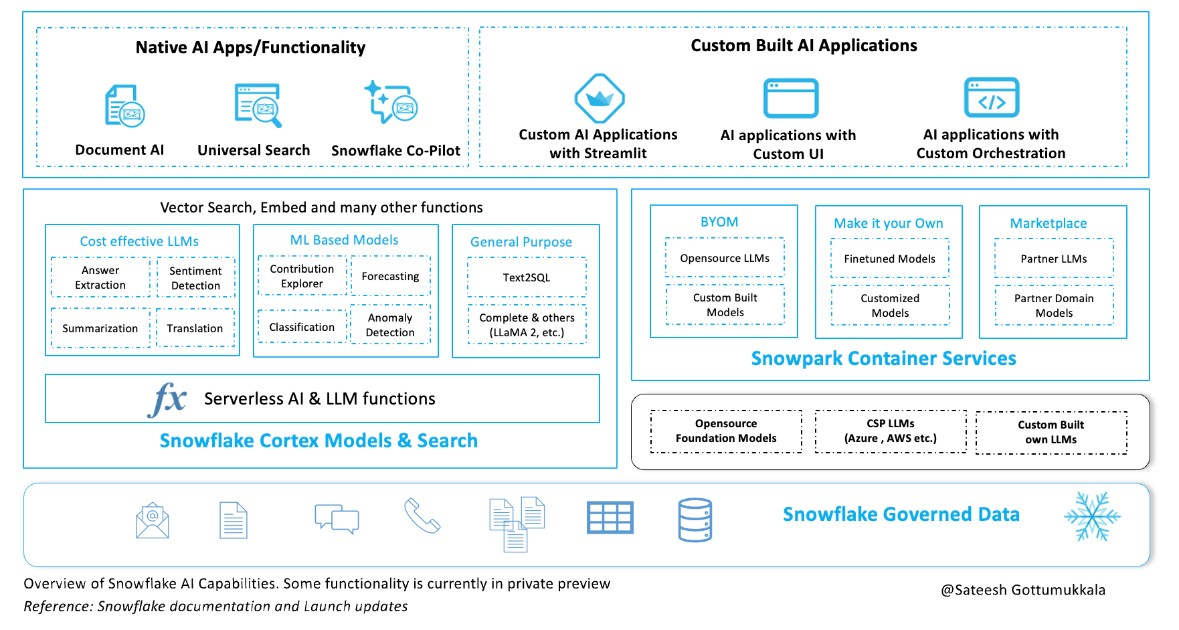
\includegraphics[width=0.85\textwidth]{images/cortexarchii.jpg}
\caption{Snowflake Cortex : fonctions IA intégrées à l'entrepôt de données}
\label{fig:cortex}
\end{figure}

Cortex propose un ensemble de fonctions couvrant les besoins courants en traitement du langage naturel : génération de texte par LLM (\texttt{CORTEX.COMPLETE}), calcul d'embeddings vectoriels (\texttt{CORTEX.EMBED\_TEXT}), résumé automatique (\texttt{CORTEX.SUMMARIZE}), traduction (\texttt{CORTEX.TRANSLATE}), analyse de sentiment (\texttt{CORTEX.SENTIMENT}), classification zero-shot (\texttt{CORTEX.CLASSIFY\_TEXT}) et extraction de réponses (\texttt{CORTEX.EXTRACT\_ANSWER}). Le tableau \ref{tab:cortex_fonctions} en présente les principales.

\begin{table}[h!]
\centering
\begin{tabularx}{\textwidth}{|l|X|X|}
  \hline
  \textbf{Fonction} & \textbf{Description} & \textbf{Cas d'usage typique} \\
  \hline
  \texttt{CORTEX.COMPLETE()} & Génération de texte par LLM. Supporte les modèles \texttt{mistral-large2}, \texttt{llama3.1-70b}, \texttt{llama3.1-8b}, \texttt{mixtral-8x7b}, etc. & Classification, extraction d'entités, génération de résumés structurés \\
  \hline
  \texttt{CORTEX.EMBED\_TEXT()} & Calcul du vecteur d'embedding d'un texte. Retourne un objet vectoriel natif. & Encodage de tickets, similarité sémantique, recherche $k$-NN \\
  \hline
  \texttt{CORTEX.SUMMARIZE()} & Génération d'un résumé concis d'un texte long. & Résumé de descriptions, synthèse de fils de discussion \\
  \hline
  \texttt{CORTEX.TRANSLATE()} & Traduction vers une langue cible (30+ langues). & Normalisation des tickets multilingues \\
  \hline
  \texttt{CORTEX.SENTIMENT()} & Analyse du sentiment, score continu entre $-1$ et $1$. & Priorisation par ton, détection d'insatisfaction \\
  \hline
  \texttt{CORTEX.CLASSIFY\_TEXT()} & Classification zero-shot sans entraînement préalable. & Triage de premier niveau \\
  \hline
  \texttt{CORTEX.EXTRACT\_ANSWER()} & Extraction de réponse à une question depuis un texte. & Extraction d'informations clés depuis une description d'incident \\
  \hline
\end{tabularx}
\caption{Fonctions LLM de Snowflake Cortex}
\label{tab:cortex_fonctions}
\end{table}

Snowflake Cortex intègre également un support natif des types vectoriels. Le type de données \texttt{VECTOR(FLOAT, n)} permet de stocker des vecteurs denses de dimension $n$, et des fonctions de similarité vectorielle (\texttt{VECTOR\_COSINE\_SIMILARITY}, \texttt{VECTOR\_L2\_DISTANCE}, \texttt{VECTOR\_INNER\_PRODUCT}) permettent d'implémenter la recherche des plus proches voisins directement en SQL, sans bibliothèque externe ni infrastructure dédiée.

\subsection{Comparaison des approches d'inférence LLM}

Trois grandes approches permettent d'intégrer des capacités LLM dans un pipeline de données. Le tableau \ref{tab:api_comparaison} en compare les caractéristiques essentielles.

\begin{table}[h!]
\centering
\begin{tabularx}{\textwidth}{|l|X|X|X|}
  \hline
  \textbf{Critère} & \textbf{Snowflake Cortex} & \textbf{APIs externes (OpenAI, Anthropic)} & \textbf{Bibliothèques locales (HuggingFace)} \\
  \hline
  Sortie de données & Non (données restent dans Snowflake) & Oui (envoi au fournisseur) & Non (tout local) \\
  \hline
  Taille des modèles & Grands modèles (70B+) & Très grands (GPT-4, Claude 3) & Limité par la RAM/GPU \\
  \hline
  Latence & Faible (réseau interne) & Variable (réseau public) & Faible (modèles légers) \\
  \hline
  Coût & Crédits Snowflake & Facturation à l'appel (tokens) & Gratuit (hors GPU) \\
  \hline
  Intégration SQL & Native & Non & Non \\
  \hline
  Conformité & Élevée & Dépend des CGU du fournisseur & Maximale \\
  \hline
\end{tabularx}
\caption{Comparaison des approches d'inférence LLM dans un pipeline de données}
\label{tab:api_comparaison}
\end{table}

\subsection{Autres plateformes intégrant l'IA}

Pour compléter l'analyse, notons que les autres grandes plateformes cloud proposent également des fonctionnalités d'IA intégrées. BigQuery ML \cite{logo:bigquery} permet d'entraîner des modèles classiques (régression, forêts aléatoires) directement depuis SQL et d'effectuer des inférences via des intégrations avec Vertex AI \cite{logo:vertex_ai}. Redshift ML \cite{logo:redshift} offre des fonctionnalités similaires via une intégration avec Amazon SageMaker AutoPilot. Databricks MLflow \cite{logo:mlflow} est un référentiel de gestion du cycle de vie des modèles (entraînement, versioning, déploiement) bien intégré dans l'écosystème Apache Spark et Delta Lake.

La différence structurante de Snowflake Cortex réside dans la disponibilité de LLM de grande taille (modèles à 70 milliards de paramètres et plus) directement accessibles depuis SQL, sans aucun déplacement des données, ce qui est déterminant dans un contexte de confidentialité et de gouvernance des données.

%------------------------9--------------------------
\section{Synthèse et justification des choix technologiques}

\subsection{Bilan comparatif global}

L'analyse des travaux existants et des technologies disponibles permet de dessiner les contours d'une architecture optimale pour notre projet. Plusieurs constats émergent de cette revue de littérature :

Premièrement, les approches classiques de classification de tickets (TF-IDF + SVM) atteignent rapidement leurs limites sur des corpus de grande taille avec une forte variabilité lexicale \cite{logo:antoniol2008, logo:lamkanfi2010}. Elles ne peuvent exploiter la richesse sémantique des descriptions de tickets ni tirer parti de la structure des données JIRA (commentaires, journal de modifications, relations inter-tickets).

Deuxièmement, le fine-tuning de modèles pré-entraînés offre de meilleures performances, mais il est coûteux en données annotées, en ressources computationnelles et en infrastructure. Dans un contexte de confidentialité des données et de délais de projet, il n'est pas la première option à envisager.

Troisièmement, l'approche RAG hybride (recherche vectorielle + arbitrage LLM) offre le meilleur compromis \cite{logo:rag, logo:advanced_rag} : elle ne nécessite pas de données annotées pour la recherche par similarité, elle est adaptable sans réentraînement, et elle produit des prédictions traçables et explicables.

Quatrièmement, l'intégration de l'IA directement dans l'entrepôt de données (via Snowflake Cortex) élimine la complexité architecturale liée à l'interopérabilité entre systèmes et garantit que les données sensibles ne quittent pas l'environnement sécurisé Snowflake \cite{logo:snowflake_cortex}.

\subsection{Justification de l'écosystème retenu}

L'ensemble technologique retenu pour ce projet repose sur quatre piliers complémentaires :

\textbf{Snowflake \cite{logo:snowflake}} comme plateforme centrale de stockage et d'analyse. Son architecture de séparation calcul/stockage, sa compatibilité SQL complète, son support natif des données semi-structurées et son intégration Cortex en font la plateforme la plus adaptée pour centraliser l'ensemble du pipeline de données et d'IA.

\textbf{dbt \cite{logo:dbt}} comme outil de transformation. Son approche SQL déclarative, ses mécanismes de test et de documentation intégrés, et sa gestion des dépendances via DAG en font l'outil le plus rigoureux pour construire un pipeline de transformation reproductible et maintenable.

\textbf{Snowflake Cortex \cite{logo:snowflake_cortex}} pour les fonctions d'IA. Il permet d'exécuter des modèles de langage (Mistral Large 2 \cite{logo:mistral}, Llama 3.1-70B \cite{logo:llama}) et de calculer des embeddings multilingues directement depuis SQL, garantissant la confidentialité des données et simplifiant l'architecture.

\textbf{Streamlit \cite{logo:streamlit}} pour la restitution. Son intégration native avec Snowflake et sa capacité à produire des interfaces interactives en Python le rendent idéal pour exposer les prédictions et les analyses aux utilisateurs finaux sans infrastructure web dédiée.

%------------------------Conclusion--------------------------
\section{Conclusion}

Ce chapitre a permis de positionner notre projet dans le panorama des technologies et des approches existantes. L'analyse des architectures Big Data nous a conduits vers Snowflake \cite{logo:snowflake} pour sa flexibilité et son intégration IA native. L'étude des paradigmes de transformation a mis en évidence la supériorité de l'approche dbt \cite{logo:dbt} pour garantir la qualité et la traçabilité des données. L'exploration des avancées en TALN et en LLM \cite{logo:transformer, logo:bert, logo:rag} a confirmé la pertinence de l'approche RAG hybride, qui combine les atouts de la recherche sémantique et de la génération augmentée sans nécessiter de réentraînement. Enfin, la comparaison des solutions d'intégration IA dans les entrepôts de données a justifié le recours à Snowflake Cortex \cite{logo:snowflake_cortex} pour ses propriétés de confidentialité et de simplicité opérationnelle. Le chapitre suivant est consacré à la conception détaillée du système, en décrivant l'architecture de la plateforme, la modélisation des données et le pipeline de classification.
